\chapter{Introduction}
%labels will help you to reference to certain images, tables, chapters, section, and so on...
\label{introduction}
%DELETEME: 
%for readability purpose, 
%it makes sense to write a short paragraph on 
%what the reader can expect in this chapter.

%DELETEME: tipp: sometimes it makes sense to 
%write the first chapter, 
%the last chapter, 
%and the abstracts at the end. 
%In this case, it might be easier to argue towards your topic



%###################################################################################
%###################### Motivation          ########################################
%###################################################################################
\section{Motivation}
%DELETEME: 
%This section is very important 
%since it argues why it is necessary 
%to take care of the problem 
%you are addressing in your work. 
%One way to do this is 
%coming from a very broad view on the problem 
%to a very detailled one. 
%This can be done by establishing 
%a chain of statements that refer to each other 
%until you reach your particular problem. 
%Doing this, you really need to take care 
%for citing every statement. 

%DELETEME: 
%Example for a chain: 
%Mobile communication gets increasingly popular in the world 
%(CITE sales on mobile communication infrastruce, 
%mobile phones, or increasing number of mobile phones contracts).
%$\rightarrow$ Especially smartphones, 
%which represent the next generation cellular phone (CITE), 
%get more and more used for communicating 
%not only with other people 
%but also for connecting to the Internet 
%for using various services (CITE). 
%$\rightarrow$ Smartphone are comprehensive cellular phones 
%that provide additional functionality 
%due to their increased connection 
%and processing capabilities (CITE). 
%$\rightarrow$ Most smartphones 
%offer an online application store 
%for adding software to the devices 
%which helps the users to customize their devices 
%according to their needs, 
%e.g. Android Market\footnote{
%    \url{http://market.android.com}, visited on 05/08/2011
%}. $\rightarrow$ One problem about installing 
%third-party software is that not all softwares 
%try to help the user; 
%$\rightarrow$ software with malicious intentions, 
%so called malicious software (malware), 
%can be a severe threat to smarpthone users. 
%Some malwares delete files (EXAMPLE + CITE or footnote with URL) 
%or even destroy devices (EXAMPLE + CITE or footnote with URL). 
%$\rightarrow$ More and more smartphone malwares 
%appeared in the last years (CITE). 
%$\rightarrow$ Signature-based approaches 
%work efficiently on known malware (CITE) 
%but face serious drawbacks regarding unknown malware. 
%$\rightarrow$ Oberheide et al.~\cite{oberheide:2008:cloudav} 
%state that virus engines need an average time of 48 days 
%until their databases get updated to be able to detect 
%a certain unknown malware. 
%$\rightarrow$ This in turn means that 
%smartphone users stay unprotected for this time 
%which can be seen as a severe threat. 
%$\rightarrow$ Therefore, approaches are needed 
%that are capable of detecting unknown malware for 
%protecting the users against such threats.

%DELETEME: 
%This example showed how one could argue 
%that alternative approaches for malware detection is required. 
%The length of the motivation depends on the topics handled 
%and can of course be longer. 
%The principle I am describing is also shown on Figure~\ref{fig:writing}
%\begin{figure}
%\centering
%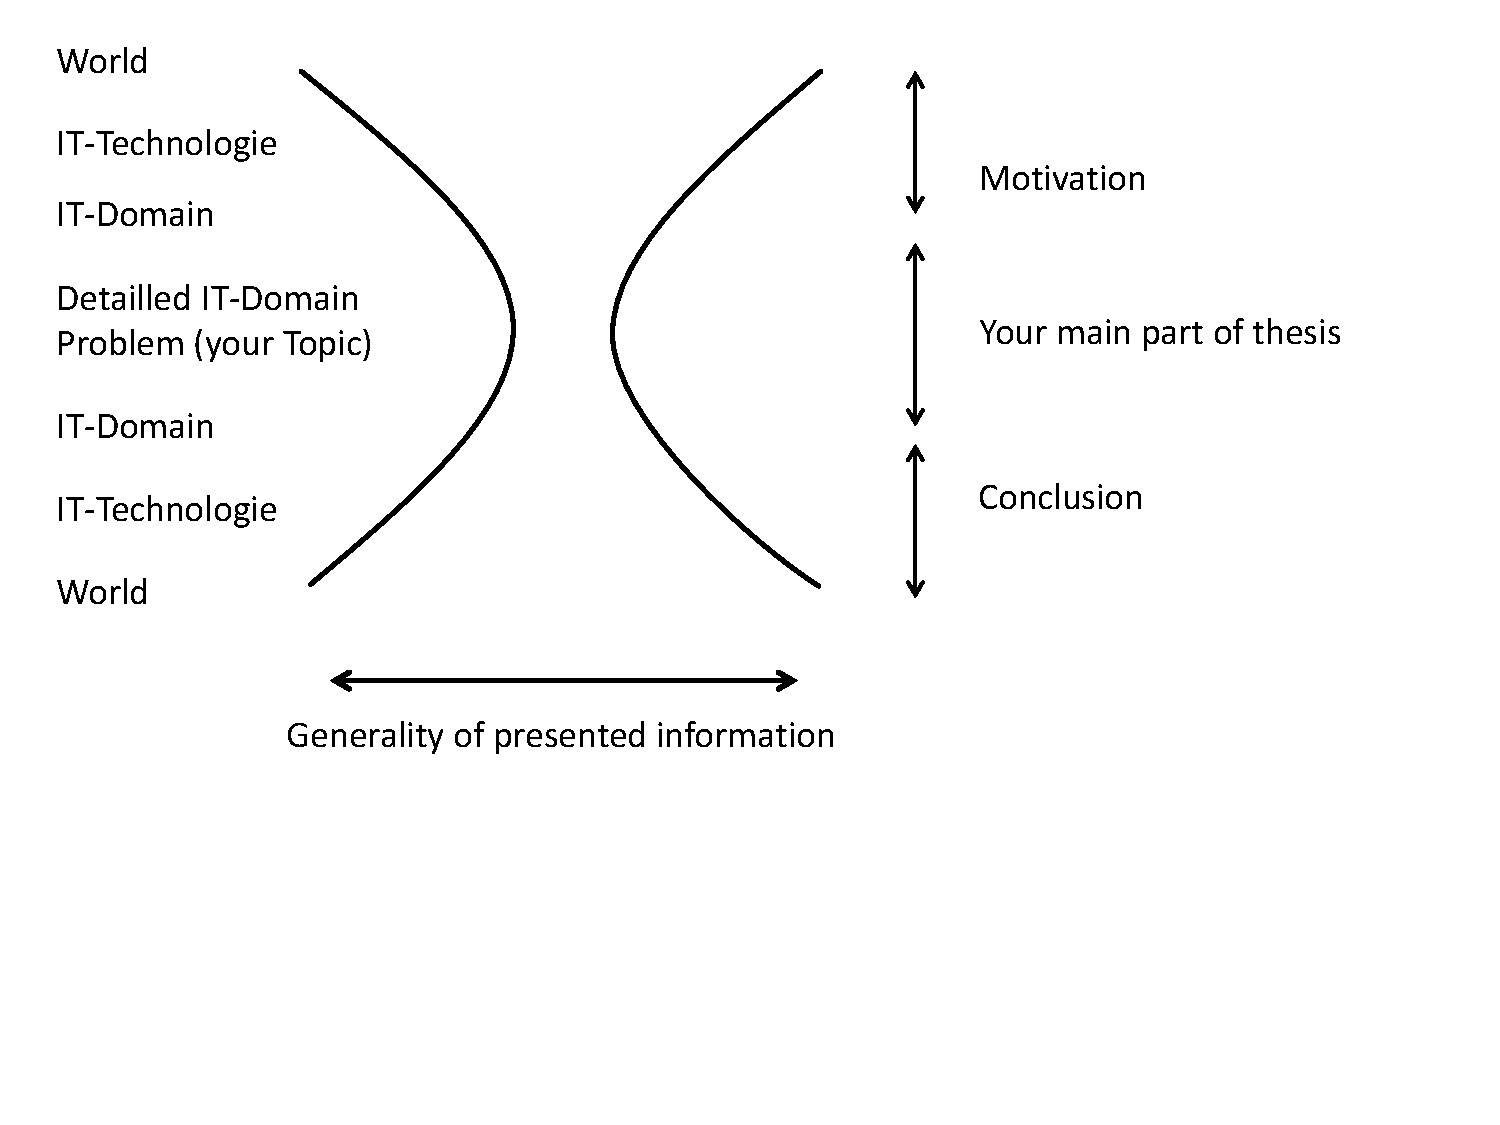
\includegraphics[width=0.9\textwidth]{template/writing}
%\caption[Information Generality]{This images illustrates how generality of information could be handled in a thesis. In your motivation you should start from a very broad view on the topic. Then you should get more precise with every statement until you reach the actual problem you are addressing. You should do vice-versa in your conclusion, starting with the problem that you addressed and getting broader until you can write about the meaning of your results to the (IT-)world.\label{fig:writing}}
%\end{figure}



Advances in drone technology in recent years
have opened the door to many civilian application possibilities,
especially in the commercial sector \cite{Dunn}.
Today, drones are already standard in 
aerial inspection services
\cite{Cohn, Equinox, Abuhasira}.
In the near future, the areas of
infrastructure,
transport,
insurance,
media and entertainment,
telecommunication,
agriculture,
safety
and mining 
are particularly promising for drones \cite{Mazur2016a}.
In contrast, 
genuine breakthroughs of more visionary applications, 
such as drone delivery or drone taxis,
are, if at all, only expected in the more distant future \cite{Rosen2019}.
Reasons for this are strict
regulations, skeptical public attitudes
and technical problems \cite{Rosen2019}.
Regarding the latter,
autonomous navigation methods are not yet 
robust enough for the reliable deployment in 
open-world environments of high uncertainty such as
densely populated urban areas \cite{brunner2019urban}.
This makes the autonomous navigation of drones
of great importance in current research.
Loquercio and Scaramuzza \cite{Loquercio2018a} 
categorize existing autonomous navigation methods for drones 
into classical methods and modern, machine learning based methods.

Classical autonomous navigation methods
follow the scheme of mapping-localization-planning-tracking.
Simpler approaches track pre-programmed waypoints based on GNSS
and are thus limited to flight environments that
first, have a reliable GNSS signal
(which often is not the case for 
urban areas, mountains, indoor sites, caves, etc.)
and second, are free of obstacles,
since functions to cope with them are absent.
More complex approaches use SLAM algorithms
to generate a map of the flight environment
and localize in it
based on the drone's visual or range sensors. \cite{MurArtal2015}
Path planning algorithms 
(e.g., \cite{Bircher2016}, \cite{Cieslewski2017})
apply to generate collision-free 
trajectories through the generated maps,
which are tracked
while estimating the drone state
based on data from the drone's inertial measurement unit (IMU)
and the output of SLAM algorithms 
(e.g., \cite{Lin2017}, \cite{Scaramuzza2014}, \cite{Sa2018}, \cite{Loianno2017}).
Theoretically, these approaches are deployable
in uncontrolled environments with unknown obstacles and other agents.
Practically, 
the mapping coerces global consistency,
which likely makes computations too complex 
for real-time execution onboard drones,
especially for non-static environments.

Modern autonomous navigation methods use machine learning
to replace the classical mapping-localization 
(or even the planning and tracking for more end-to-end methods) 
with the perception of the drone's onboard sensors
(e.g., camera, range, IMU)
and the decision-making of an ANN.
The way of learning further subdivides these methods into
reinforcement learning (RL) and imitation learning (IL) based methods.
In RL, the ANN learns with ``trial-and-error" \cite{Sadeghi2016}
from direct environmental interactions 
and thus avoids ``distributional mismatch" \cite{RobotAutonomy2}  
of training vs. testing, which is typical in IL.
However, this comes with the expense of a
substantially higher sample complexity 
compared to IL. \cite{Zhu2017}
This disadvantage is severe for drones because 
their limited flight endurance 
makes the learning process inefficient 
and collisions are uncontrolled and 
hence costly and dangerous. \cite{Sadeghi2016}

A popular research playground is autonomous drone racing
(e.g., \cite{Moon2019}, \cite{Jung2018}, \cite{Song2021})
because of the controlled flight environment,
the straightforward definition of goals
and the measurability and comparability of performance.
Methods for autonomous drone racing usually
integrate feedforward
convolutional neural networks (CNN) 
to map the current color or depth image to action
(e.g., \cite{RojasPerez2020}, \cite{Kaufmann2019}, \cite{Jung2018a}).
CNNs already achieve 
a high, spatial comprehension of how the drone's sensors perceive
the immediate environment.
However, this alone may not
be enough for the long-term objective of safely 
applying autonomous drones in open-world environments.
As humans are able to navigate safely there,
it seems promising to learn human-like abilities.
Temporal comprehension,
besides spatial comprehension,
has an important function in human navigation. 
For example, 
after entering a room through a door, 
a person can leave the room knowing 
that the door is behind him and 
does not need to keep the door in sight to do so.
Further, a person requires 
observing a sequence of images to
estimate the velocity and motion direction of herself or himself, 
obstacles or other agents.
In machine learning, recurrent neural networks
can establish temporal connections.
It is interesting to research the 
effect of using recurrent neural networks in autonomous drone racing.




%The controlled environment of autonomous drone racing 
%represents a convenient ground
%for basic research on autonomous navigation of drones
%because it clearly defines high-level goals, 
%i.e., to complete the racetrack,
%as well as intermediate goals, i.e., to fly through the next race gate.
%Moreover, the attainment of these goals can be intuitively assessed,
%for example, by considering the racetrack completion vs. the 
%maximum speed.





%The performance and robustness of different methods 
%can be assessed intuitively. 
%by means of 
%Moreover, several metrics to measure performance are provided,
%e.g., 
%
%high-level goals
%(i.e., completing the racetrack as fast/robust as possible)
%are defined and their 
%attainment can be measured (e.g., racetrack completions, flight time).
%Moreover, the racing environment is controlled
%and obsticles are known.

%Advanced methods for autonomous navigation of MAVs
%integrate feedforward, 
%deep convolutional neural networks (CNN)
%that, with a high spatial comprehension of the MAV's immediate surrounding, 
%map the current color or depth image to prediction or action.


%Consequently, 
%whether the state of the art in autonomous navigation of UAVs
%is sufficiently robust depends on the flight environment and the flight mission.
%Again, drone delivery provides an explanatory example here.
%Projects have been already 
%realized in rural areas where the airspace is mainly undisturbed [].
%Here, navigating through waypoints only relying on GNSS 
%without any implementation of obstacle avoidance and agent-coordination may be sufficient. 
%In contrast, urban areas are full of unstructered obstacles and other participating agents 
%which result in a high uncertainty that cannot be faced with in-advance planning. 
%Only a high level of autonomy in navigation
%could robustly cope with the challenges of this environment.
%This level has not yet been achieved.


%Research on autonomous MAV navigation mainly relies on deep learning 
%which allows to comprehend the immediate environment based on the perception of
%onboard sensors. \cite{loquercio2018learning}
%State-of-the-art navigation methods 
%achieve a high spatial understanding of the environment
%by feeding convolutional neural networks with RGB or depth data.
%This research aims to develop a simple navigation method 
%that extend this spatial perception onto temporal extension 
%by serially connecting a CNN with a long-short-term-memory (LSTM) network.
%Based on my assumption that powers of recall are crucial for humans when navigating,
%I am convinced that future autonomous navigation systems will also encompass this ability.
%The navigation method will be tested in simulation and real world in a simplified test scenario,
%which, however, requires the MAV to remember the expansion and relative motion of obstacles while considering its own elapsed acceleration.



%###################################################################################
%###################### Approach and Goals  ########################################
%###################################################################################
\section{Approach and Goals}
%DELETEME: 
%In this section, 
%you should cleary describe 
%your approach 
%that you are following 
%in order to solve 
%the underlaying problem 
%of your thesis. 
%Additionally, you should clearly state 
%the goals of your work. 
%This will not only help you supervizor 
%to understand what you are doing, 
%it will also help you to be sure 
%on which topic you should evaluate.



This thesis aims to 
investigate
whether temporal comprehension 
induced by a recurrent neural network
can be beneficial for
autonomous navigation in drone racing.
To do this, the thesis uses
the vision-based autonomous navigation method
proposed by Kaufmann et al. \cite{Kaufmann2018} as a baseline.
In the tests conducted by the authors, the baseline method
stood out from the compared methods
with high reliability and agility 
along dynamic flight curves through the racetrack.
The baseline method has a hybrid structure:
an artificial neural network 
inferring navigation decisions 
from the images of the drone's onboard camera
and a planning-control stack 
translating these decisions into flight movement.
The baseline ANN is a serial connection
of a convolutional neural network (CNN) 
and fully connected (FC) layers.
The CNN extracts visual features from imagery,
enabling the baseline method
to comprehend spatially what is in view of 
the drone's onboard camera.

This thesis extends the baseline ANN
with a multi-layer gated recurrent unit (GRU).
Theoretically, this
recurrent neural network variant 
enables the autonomous navigation method
to remember and to establish temporal connections.
Specifically, this means that navigation decisions 
base on both current and past sensor data.
Considering that, first, 
navigation can be seen as 
sequentially making decisions 
regarding how to move through space, and second, 
the thereby resulting trajectories 
are 4D objects in space and time, 
the CNN-GRU approach of this thesis, 
by incorporating both spatial and temporal understanding, 
likely improves race performance.
This thesis investigates this hypothesis in simulated drone races.
Different variants of ANNs 
are tested for their performance 
at different maximum speeds 
and for their ability to cope 
with intermediate target loss.
The latter refers to the event
that the next race gate leaves the FOV of the drone's camera
(e.g., because of a sharp turn between two race gates)
and the drone can only make meaningful navigation decisions
based on the memory induced by the GRU.







%According to the paper, the baseline has a success rate of 100 \% on the simulated racetrack when 
%the maximum speed is not greater than 9 m/s. For higher maximum speeds
%\{10, 11, 12\} m/s the success rate decreases to approximately \{85, 60, 35\} \%.
%Besides maximum speed, the simulated racetrack is designed in way that at any time the 
%currently targeted race gate is located in the frame of view (FOV) of the onboard camera.
%This is a requirement of the baseline because the CNN derives its navigation decisions only
%from the current image. In the event of intermediate target loss, i.e.,
%there is no race gate in the FOV and, consequently, on the image, the baseline 
%must result in undefined behaviour. 
%Intermediate target loss could for example 
%happen in the case of a steep curve between two consecutive race gates
%or in the case of an obstacle that temporally blocks the view to the currently targeted gate.
%In my thesis I plan to further develop only the first part of the hybrid approach.
%I intend to, first, replace the CNN with a R-CNN and,
%second, feeding additional features, i.e., data from the inertial measurement unit (IMU), to the network.
%The IMU data encompasses three (x, y, z) linear accelerations and three (x, y, z) angular velocities.
%I expect that thereby, 
%waypoints are not only generated on the basis of the current RGB image and IMU data, 
%but that also past sensor data is included in the navigation decision.
%This would possibly result in the following positive effects:
%\begin{itemize}
%	\item Making decisions on the basis of a series of sensor data makes the network more robust against outliers.
%			Otherwise, at high speeds, outliers may directly result in a crash.
%	\item Considering the similarity of recurrency to mathematical integration,
%			feeding IMU data to the network could have great potential since the network could be more or less able to internally estimate positions and orientations.
%	\item Due to its "memory", the network is able to generate meaningful waypoints in the case of intermediate target loss, i.e.,
%			the next gate of the race track is not depicted in the current image, but has appeared in previous images.
%	%\item Due to temporally distributed images, the network is able to take the speeds of moving gates (or obstacles) into the account of the navigation decisions.
%	\item Because trajectories are temporally extended maneuvers, a network with temporal comprehension is more able to imitate the expert system.
%			Thus, the resulting trajectory through the race track formed 
%			by the successively generated waypoints 
%			is more similar to a precomputed optimal trajectory.
%\end{itemize}
%The approach is implemented utilizing the middleware ROS \cite{ros}
%and simulated with the photo-realistic Flightmare Simulator \cite{song2020flightmare} built on Unity.
%For the implementation concept, see section \ref{sec:implConcept}.
%In simulation, the following tests should be conducted to compare my approach to the baseline.





%\paragraph{Randomized Figure-8 Drone Racing}
%Conduct test runs with increasing maximum speeds.
%For each run,
%build a randomized figure-8 drone racing track
%and test my approach and the baseline on the track.
%For each maximum speed, evaluate the percentage share of successful runs,
%the average time of racetrack completion
%and the
%closeness to the global trajectory in terms of optimality.
%The latter could be computed by recording the reference states
%that are continually pushed to the autopilot,
%taking the 4th derivative with respect to time (snap)
%and integrate the values.
%The in this way calculated cost could be used to measure closeness to
%the optimal, minimum snap global trajectory which the expert system used to generate the 
%training data.


%\paragraph{Intermediate target loss on sharp curve}
%Simulate two gates with a sharp curve in between.
%Before the drone passes the first gate,
%both successive gates must appear in the frame of view of the onboard camera.
%The curve must be so sharp, that, after traversing the first gate, not only the first but also the second gate has left the frame of view.
%The baseline, whose CNN makes navigation decisions from only the current image, will likely to fail in this scenario
%due to the absence of a goal.
%In contrast, my approach uses an R-CNN which is able to internally store information from previous images.
%In case that the R-CNN is well trained, it should be able to generate meaningful waypoints to complete the sharp curve and traverse the second gate.
%This becomes especially true, if the R-CNN is able to make use of the IMU data estimating poses.
%The percentage share of successful runs would be a convenient metric for evaluation.


%###################################################################################
%###################### Structure of the Thesis ####################################
%###################################################################################
\section{Structure of the Thesis}
%DELETEME: 
%This section does not require eloquent writing.
%It is just a presentation of what you will handle 
%in each chapter starting with Chapter~\ref{background}.

%DELETEME: Example: 
%This thesis is structured as follows. 
%In Chapter~\ref{background}, 
%we discuss essential background related to the thesis topic. 
%(SOME MORE SENTENCES). 
%Chapter~\ref{mainone} represents 
%a detailled analysis of the problem 
%that will be addressed. In particular, (SOME MORE SENTENCES). 
%In Chapter~\ref{maintwo}, 
%our solution is presented. 
%This solution covers ... (SOME MORE SENTENCES). 
%Chapter~\ref{evaluation} evaluates our solution 
%basing on our specified goals. 
%(SOME MORE SENTENCES). 
%In Chapter~\ref{conclusion}, we conclude. 
%Chapter~\ref{appendices} gives additional related information 
%on the topic of this thesis.



%DELETEME: Example: 
Chapter~\ref{background}
provides background information on the thesis topic,
including imitation learning with dataset aggregation
and the gated recurrent unit architecture.
Chapter~\ref{mainone} presents
the baseline autonomous navigation method
comprising the ANN module, 
the planning module, the control stack and the expert system.
Special attention is paid to the ANN module,
which extends the baseline ANN with the temporal comprehension of the GRU.
Chapter~\ref{maintwo} presents the design of the
experiments conducted in this thesis,
including the simulation setup,
the imitation learning process and the race tests.
Chapter~\ref{evaluation} evaluates 
the experimental results
focussing on the impact of temporal comprehension on performance.
Chapter~\ref{conclusion} concludes this thesis. 
Chapter~\ref{appendices} provides additional related information.